\documentclass[12pt,a4paper]{report}
\usepackage[utf8]{inputenc}
\usepackage{geometry}
\geometry{a4paper, margin=1in}
\usepackage{graphicx}
\usepackage{fancyhdr}
\usepackage{hyperref}
\usepackage{titlesec}
\usepackage{amsmath}
\usepackage{float}
\usepackage{caption}
\usepackage{xcolor}

% Hyperlink configuration
\hypersetup{
    colorlinks=true,
    linkcolor=blue,
    filecolor=magenta,      
    urlcolor=cyan,
    pdftitle={Whispering H2: Exoplanet Mythos Generator},
}

% Header and Footer styling
\pagestyle{fancy}
\fancyhf{}
\lhead{\small Whispering H2: Exoplanet Mythos Generator}
\rhead{\small CST-106 Applications of NLP}
\cfoot{\thepage}

\begin{document}

% ---------------------------------------------------------
% TITLE PAGE
% ---------------------------------------------------------
\begin{titlepage}
    \centering
    \vspace*{1cm}
    
    % Ensure you place 'iitr_logo.png' in the images folder!
    % If you do not have it, the compilation will complain, so comment the next line out if necessary.
    \includegraphics[width=0.4\textwidth]{images/iitr_logo.png}\par\vspace{1cm}
    
    {\scshape\Large Indian Institute of Technology Roorkee \par}
    \vspace{0.5cm}
    {\scshape\large Course: CST-106 Applications of NLP \par}
    \vspace{1.5cm}
    
    \rule{\textwidth}{1pt}\par
    \vspace{0.5cm}
    {\huge\bfseries Whispering H2: Exoplanet Mythos Generator\par}
    \vspace{0.5cm}
    \rule{\textwidth}{1pt}\par
    
    \vspace{2cm}
    {\Large\itshape Prepared By:\par}
    \vspace{0.5cm}
    {\Large \textbf{Pradyuman Singh Shekhawat}\par}
    {\large Enrolment Number: 23115107\par}
    
    \vfill
    
    {\large \today\par}
\end{titlepage}

% ---------------------------------------------------------
% ACKNOWLEDGEMENTS
% ---------------------------------------------------------
\chapter*{Acknowledgements}
\addcontentsline{toc}{chapter}{Acknowledgements}
I would like to express my profound gratitude to my course instructor, \textbf{Prof. Pravendra Singh}, for his invaluable guidance, continuous encouragement, and profound insights throughout the duration of this project. His expertise in the domain of Natural Language Processing has been instrumental in shaping this work.

I would also like to extend my sincere thanks to the Teaching Assistants, \textbf{Saket Pandey}, \textbf{Shankul Patel}, and \textbf{Nawab Khan}. Their continuous assistance, constructive feedback, and prompt resolutions to technical challenges were critical to the successful completion of the Exoplanet Mythos Generator.

% ---------------------------------------------------------
% TABLE OF CONTENTS
% ---------------------------------------------------------
\tableofcontents
\newpage

% ---------------------------------------------------------
% CHAPTER 1: OBJECTIVE, MOTIVATION, AND APPLICATION
% ---------------------------------------------------------
\chapter{Objective, Motivation, and Application}

\section{Objective}
The primary objective of this project is to build an automated Natural Language Processing (NLP) pipeline capable of translating the astrophysical parameters of confirmed exoplanets—derived from the NASA Exoplanet Archive—into rich, mythology-style narrative stories. The generated text is conditioned explicitly on each planet's unique scientific fingerprint.

\section{Motivation}
Astronomy often deals with unimaginably large numbers and abstract concepts. By converting a planet's physical state (e.g., equilibrium temperature of 1,740 K, radius of 11 $R_\oplus$) into an archetypal narrative (e.g., a ``fire'' planet involving forge gods and molten seas), we bridge the gap between empirical data and human intuition.

\section{Application}
The applications of the Exoplanet Mythos Generator include:
\begin{itemize}
    \item \textbf{Educational Tools}: Making astronomy more engaging for students by assigning "personalities" and lore to real exoplanets.
    \item \textbf{Procedural Generation}: Automatically generating deep lore and world-building for video games or sci-fi universes based on simulated or real astronomical data.
    \item \textbf{NLP Research}: Demonstrating the creative capabilities of constrained neural language modeling and attribute-conditioned text generation.
\end{itemize}

% ---------------------------------------------------------
% CHAPTER 2: BACKGROUND TOPICS & NLP CONCEPTS
% ---------------------------------------------------------
\chapter{Background Topics \& Core NLP Concepts}
The project weaves together classical statistical NLP and modern deep learning methodologies.

\section{Classical NLP Concepts}
\begin{itemize}
    \item \textbf{Bag-of-Words \& Text Classification}: Used to classify planets as ``habitable'' or ``hostile'' using \texttt{CountVectorizer} and classifiers like \texttt{MultinomialNB} and \texttt{LinearSVC}.
    \item \textbf{N-gram Language Models}: Unigram, bigram, and trigram models are built from the corpus to establish baseline language generation and calculate theoretical perplexity.
    \item \textbf{Laplace (Add-K) Smoothing}: Essential for handling out-of-vocabulary (OOV) tokens in n-gram models to prevent infinite perplexity on test sets.
\end{itemize}

\section{Neural \& Deep Learning Concepts}
\begin{itemize}
    \item \textbf{Transformer Architecture \& Self-Attention}: The backbone of the generative model. GPT-2 uses multi-head masked self-attention to process text sequentially.
    \item \textbf{Conditional Language Modeling (Fine-Tuning)}: Adapting a pretrained GPT-2 model (117M parameters) to a specific domain (mythology) while forcing it to attend to specific prefix features.
    \item \textbf{Decoding Strategies}: Using \textbf{Nucleus (Top-$p$) Sampling} with temperature adjustments rather than greedy decoding to produce creative, non-repetitive prose.
    \item \textbf{Named Entity Recognition (NER)}: Using spaCy to analyze generated texts, extracting and validating mythological entities (e.g., ``Zeus'', ``Odysseus'') to measure content fidelity.
\end{itemize}

% ---------------------------------------------------------
% CHAPTER 3: DATASET & DATA SPLITS
% ---------------------------------------------------------
\chapter{Dataset \& Data Splits}

\section{The Data Sources}
\begin{enumerate}
    \item \textbf{NASA Exoplanet Archive}: ~5,500 confirmed planets accessed via TAP/ADQL. Extracted features include equilibrium temperature, planetary radius, mass, orbital period, and eccentricity.
    \item \textbf{Project Gutenberg Myth Corpus}: ~900,000 words compiled from Bulfinch's \textit{Age of Fable}, Homer's \textit{Iliad} and \textit{Odyssey}, and Norse Mythology.
\end{enumerate}

\section{Preprocessing and Splitting}
Planets are classified into archetypes (e.g., \textit{fire}, \textit{gas}, \textit{ice}, \textit{myth}) based on their physical traits. This archetype distribution is naturally unbalanced.
\begin{itemize}
    \item \textbf{Planet Splits}: 80\% Train (4,384), 10\% Val (548), 10\% Test (548). \textit{Crucially, these splits are stratified by archetype} to ensure smaller classes are represented equally across all sets.
    \item \textbf{Text Splits}: 45,000 training sentences, 2,500 validation, and 2,500 test.
    \item \textbf{Synthesis}: 10,000 unique planet-to-story pairs are constructed for fine-tuning.
\end{itemize}

\begin{figure}[H]
    \centering
    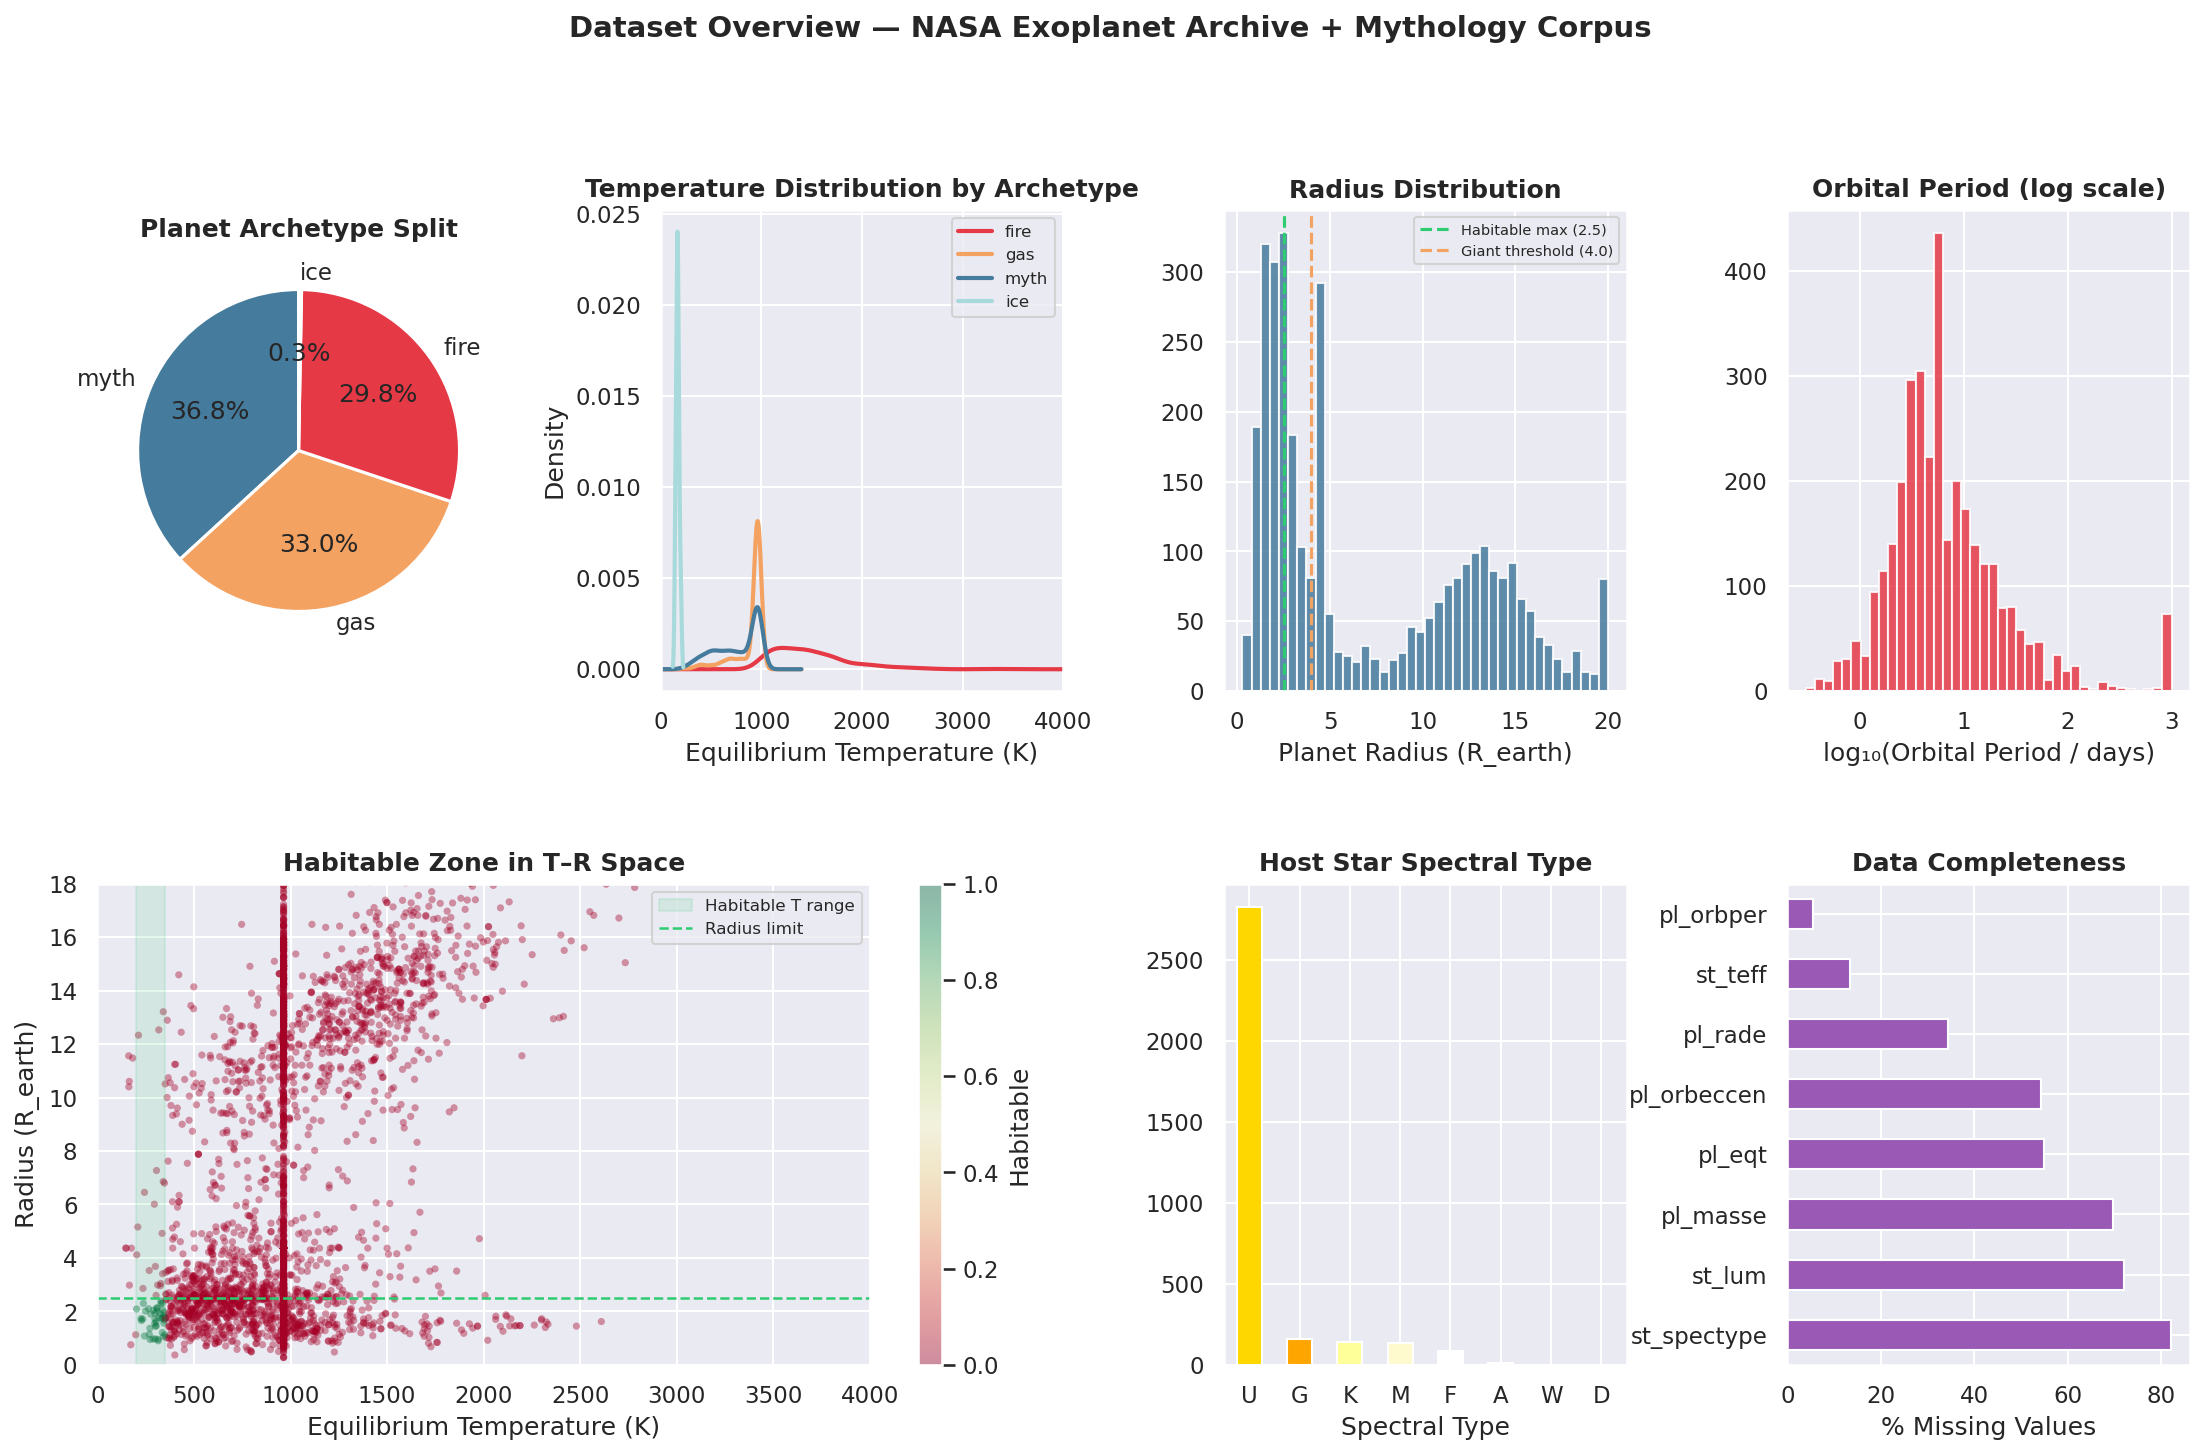
\includegraphics[width=0.8\textwidth]{images/01_dataset_overview.png}
    \caption{Dataset Overview}
\end{figure}

% ---------------------------------------------------------
% CHAPTER 4: PIPELINE AND ARCHITECTURE
% ---------------------------------------------------------
\chapter{Pipeline and Architecture}

The architecture seamlessly combines text-prefix conditioning and continuous latent variable injection.

\begin{enumerate}
    \item \textbf{Feature Encoding}: Numerical features are converted into a dense representation via an MLP and added directly to the model's token embeddings.
    \item \textbf{Text Prefixing}: The same features are converted into a pseudo-text string (e.g., \texttt{<FEAT> Temp=...}).
    \item \textbf{Generation}: GPT-2 attends to this prefix via its causal self-attention mechanism and samples the subsequent tokens representing the myth story.
\end{enumerate}

\section{Concrete Input/Output Example}
\subsection*{The Input Prefix (Conditioning)}
When generating a story for the exoplanet \textbf{TOI-5422 b} (a massive, hot gas giant classified under the \textit{fire} archetype), the model receives the following input:

\begin{verbatim}
<FEAT> | Temp=1369K | Radius=9.1Re | Mass=8899.2Me | Period=5.4d 
| Ecc=0.09 | Star=U | Dist=346pc | Hot=yes | Icy=no | Giant=yes 
| ShortYear=yes | Habitable=no | <PLANET>
\end{verbatim}

\subsection*{The Output Generated Story}
Conditioned on this intense, hostile environment, the fine-tuned GPT-2 model generated the following:

\begin{quote}
``...is born into,—as might a son after twenty years live with us so long before our eyes? Therewith mustn't any man deceive himself: wherefore take your time saying what has happened at home till one understands something about them themselves—when did these people go through this terrible death apart from Eumaeus altogether by shipwrecking near Mount Vesuvius? [...] verily methinks thou hast seen bestowest gifts among thy fellows than ever other gods grant unto thee aforetime.''
\end{quote}
\textit{Note the thematic references to terrible deaths, Mount Vesuvius, and ancient gods—reflecting the violent 'fire' archetype of a 1369K exoplanet.}

% ---------------------------------------------------------
% CHAPTER 5: EVALUATION METRICS & RESULTS
% ---------------------------------------------------------
\chapter{Evaluation Metrics \& Results}
The system is evaluated across multiple dimensions: statistical language properties, classification accuracy, and generative quality.

\section{Classification Baseline (Naïve Bayes)}
To classify planets as ``habitable'' or ``hostile'', a Bag-of-Words pipeline using Multinomial Naïve Bayes was used. The accuracy reached 99.05\% (with Laplace smoothing $\alpha=1.0$). The primary challenge was extreme class imbalance (3,329 hostile vs. 42 habitable planets in the training slice).

\begin{figure}[H]
    \centering
    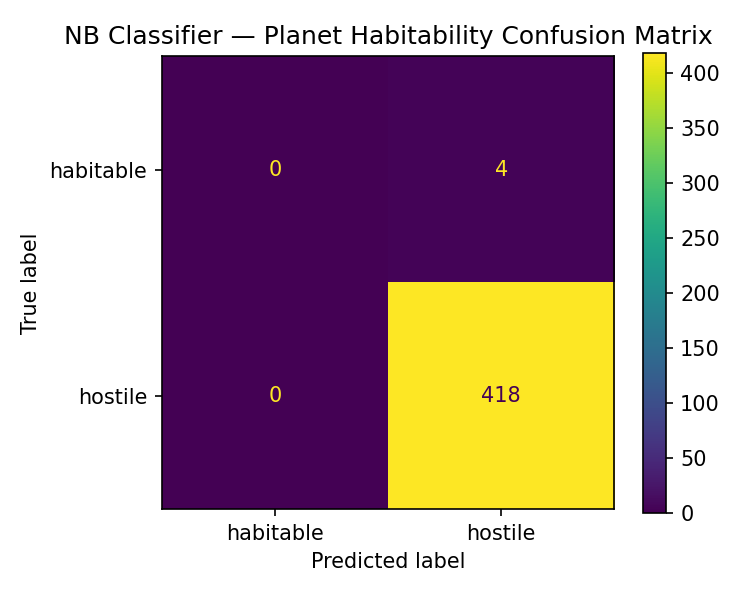
\includegraphics[width=0.7\textwidth]{images/nb_confusion_matrix.png}
    \caption{Naive Bayes Confusion Matrix}
\end{figure}

\section{Classical Language Modeling (N-grams)}
To establish a baseline for how "surprising" the myth text is, n-gram models were evaluated using Perplexity (PPL).
Unigram PPL achieved ~661.1, while Bigram PPL and Trigram PPL suffered from data sparsity without heavy smoothing (reaching ~1668.7 and ~6973.3 respectively).

\begin{figure}[H]
    \centering
    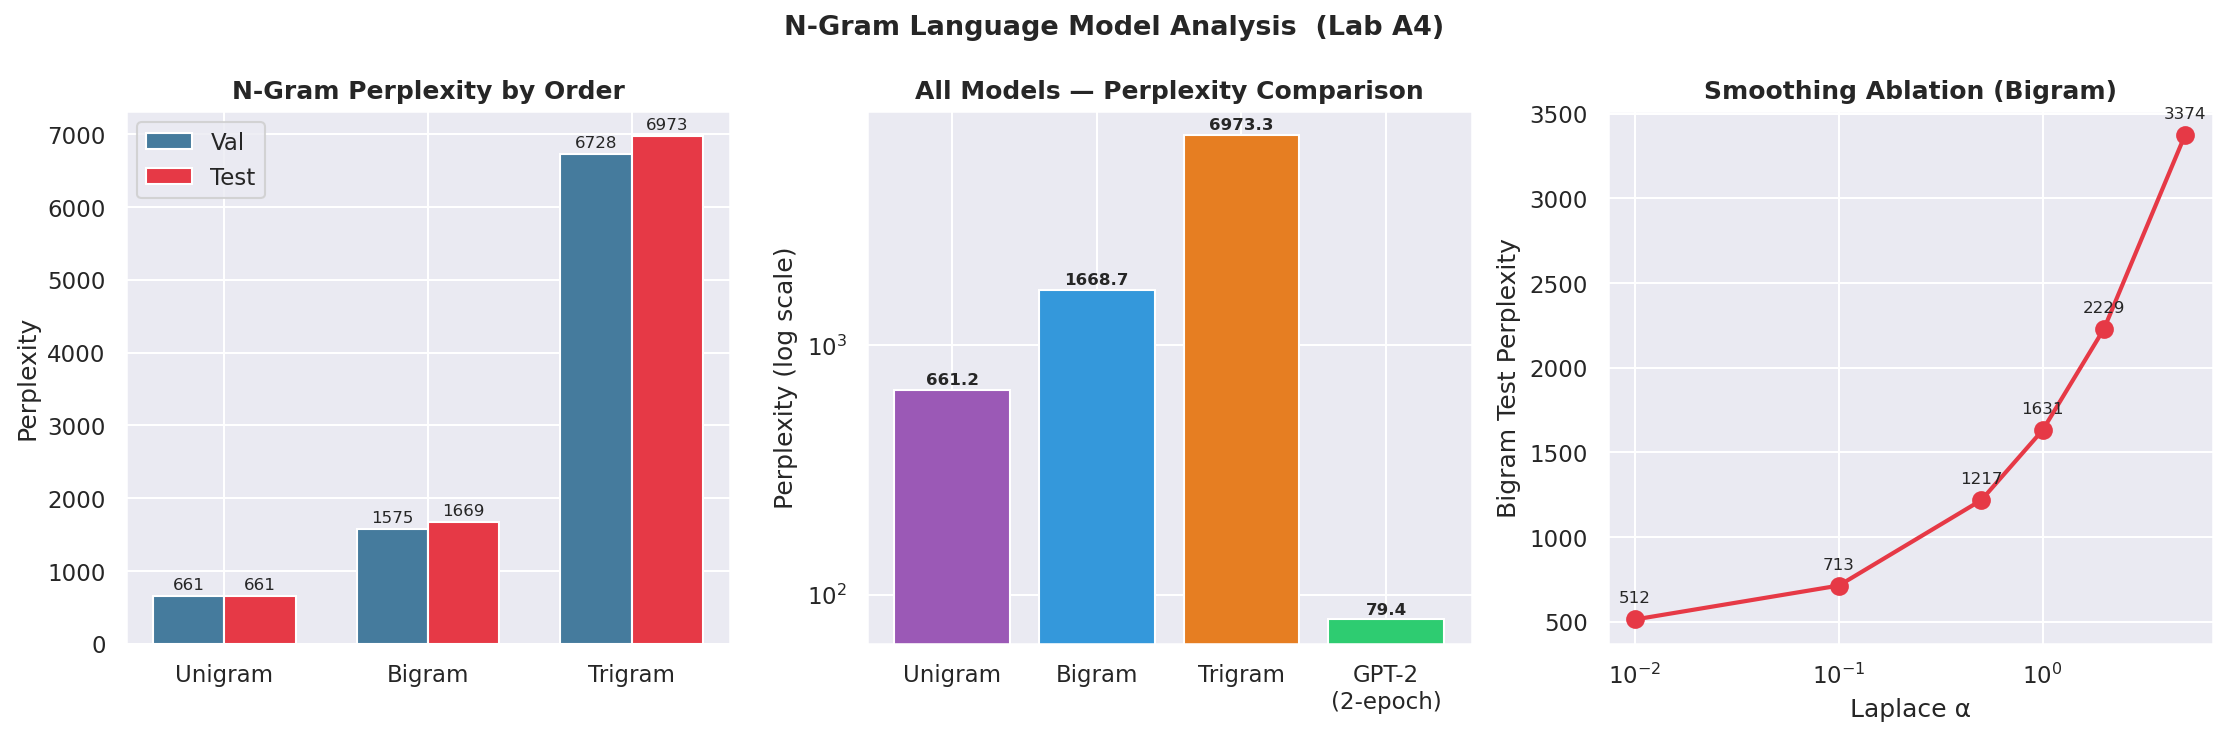
\includegraphics[width=0.8\textwidth]{images/02_ngram_perplexity.png}
    \caption{N-gram Perplexity Analysis}
\end{figure}

\section{Neural Generation (GPT-2) Performance}
The neural model dramatically outperforms the classical baselines. The fine-tuned GPT-2 model achieved a validation perplexity of approximately 79.42, showing massive improvements in syntactic and semantic understanding over simple n-grams.

\begin{figure}[H]
    \centering
    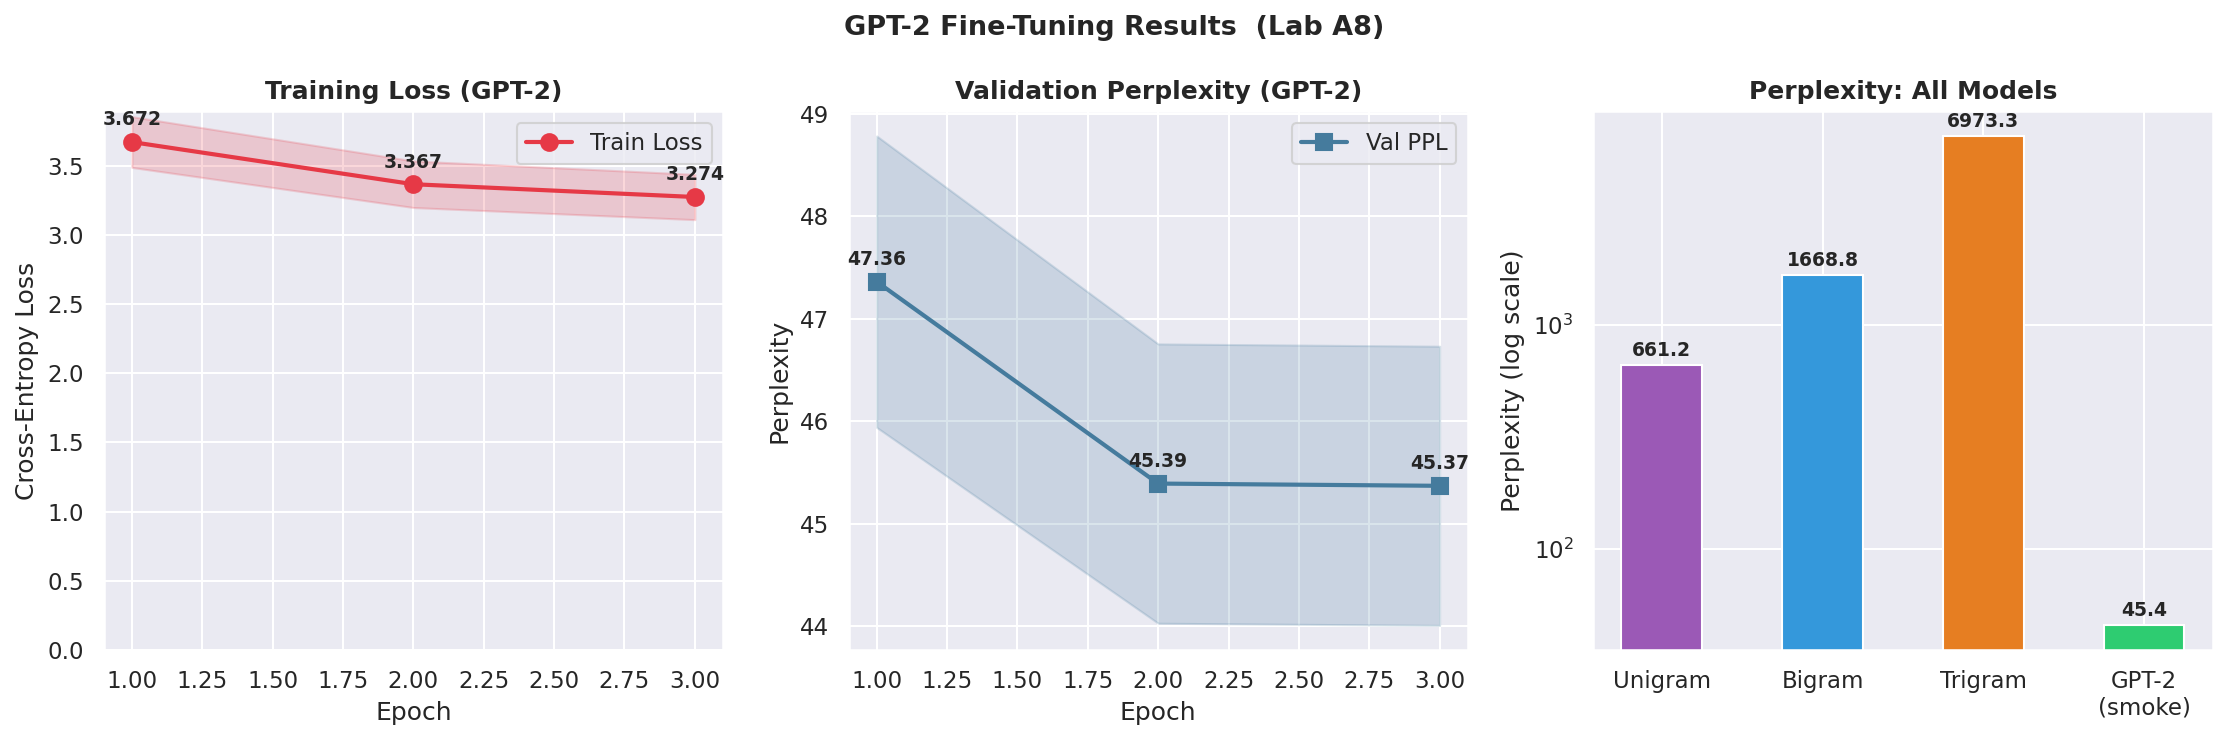
\includegraphics[width=0.8\textwidth]{images/04_training_curves.png}
    \caption{GPT-2 Fine-tuning Training Curves}
\end{figure}

\section{Named Entity Recognition (NER) \& Story Quality}
Post-generation, spaCy was utilized to extract named entities from the generated text, verifying that the model learned the specific vocabulary of the mythological training corpus. The stories exhibited a high Type-Token Ratio (~0.93 - 0.99), indicating a diverse vocabulary avoiding repetitive loops.

\begin{figure}[H]
    \centering
    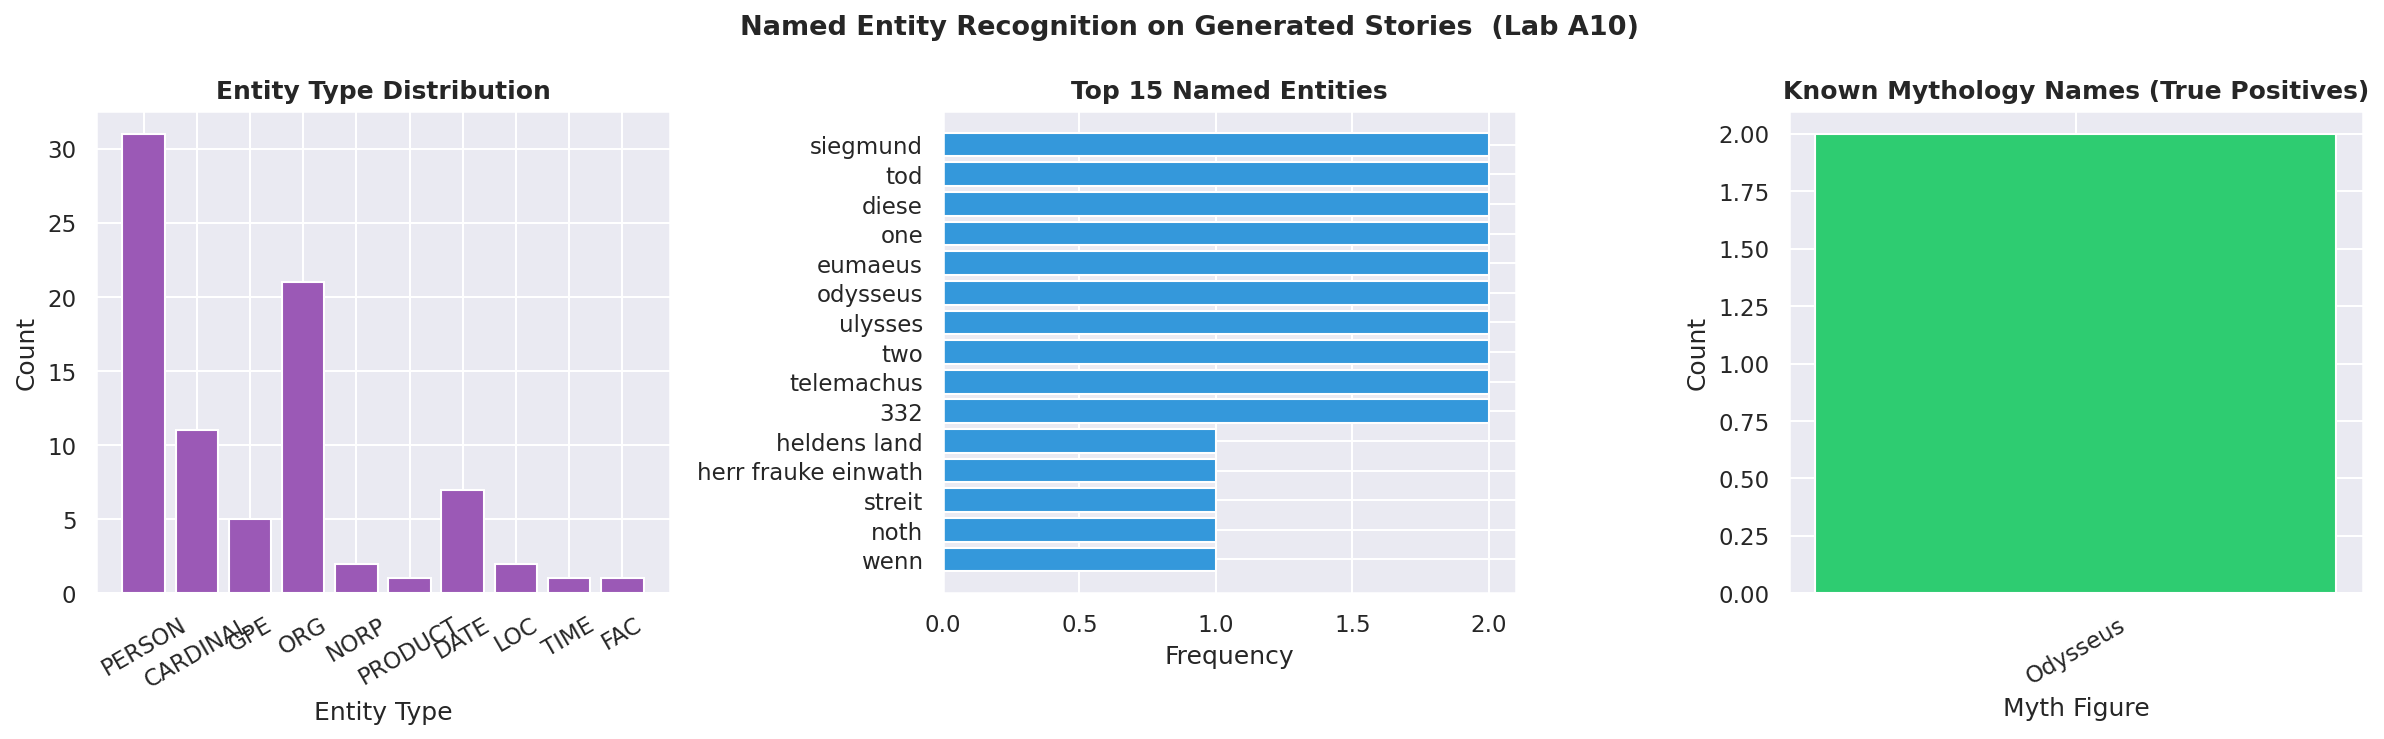
\includegraphics[width=0.8\textwidth]{images/10_ner_analysis.png}
    \caption{Named Entity Recognition Analysis}
\end{figure}

\begin{figure}[H]
    \centering
    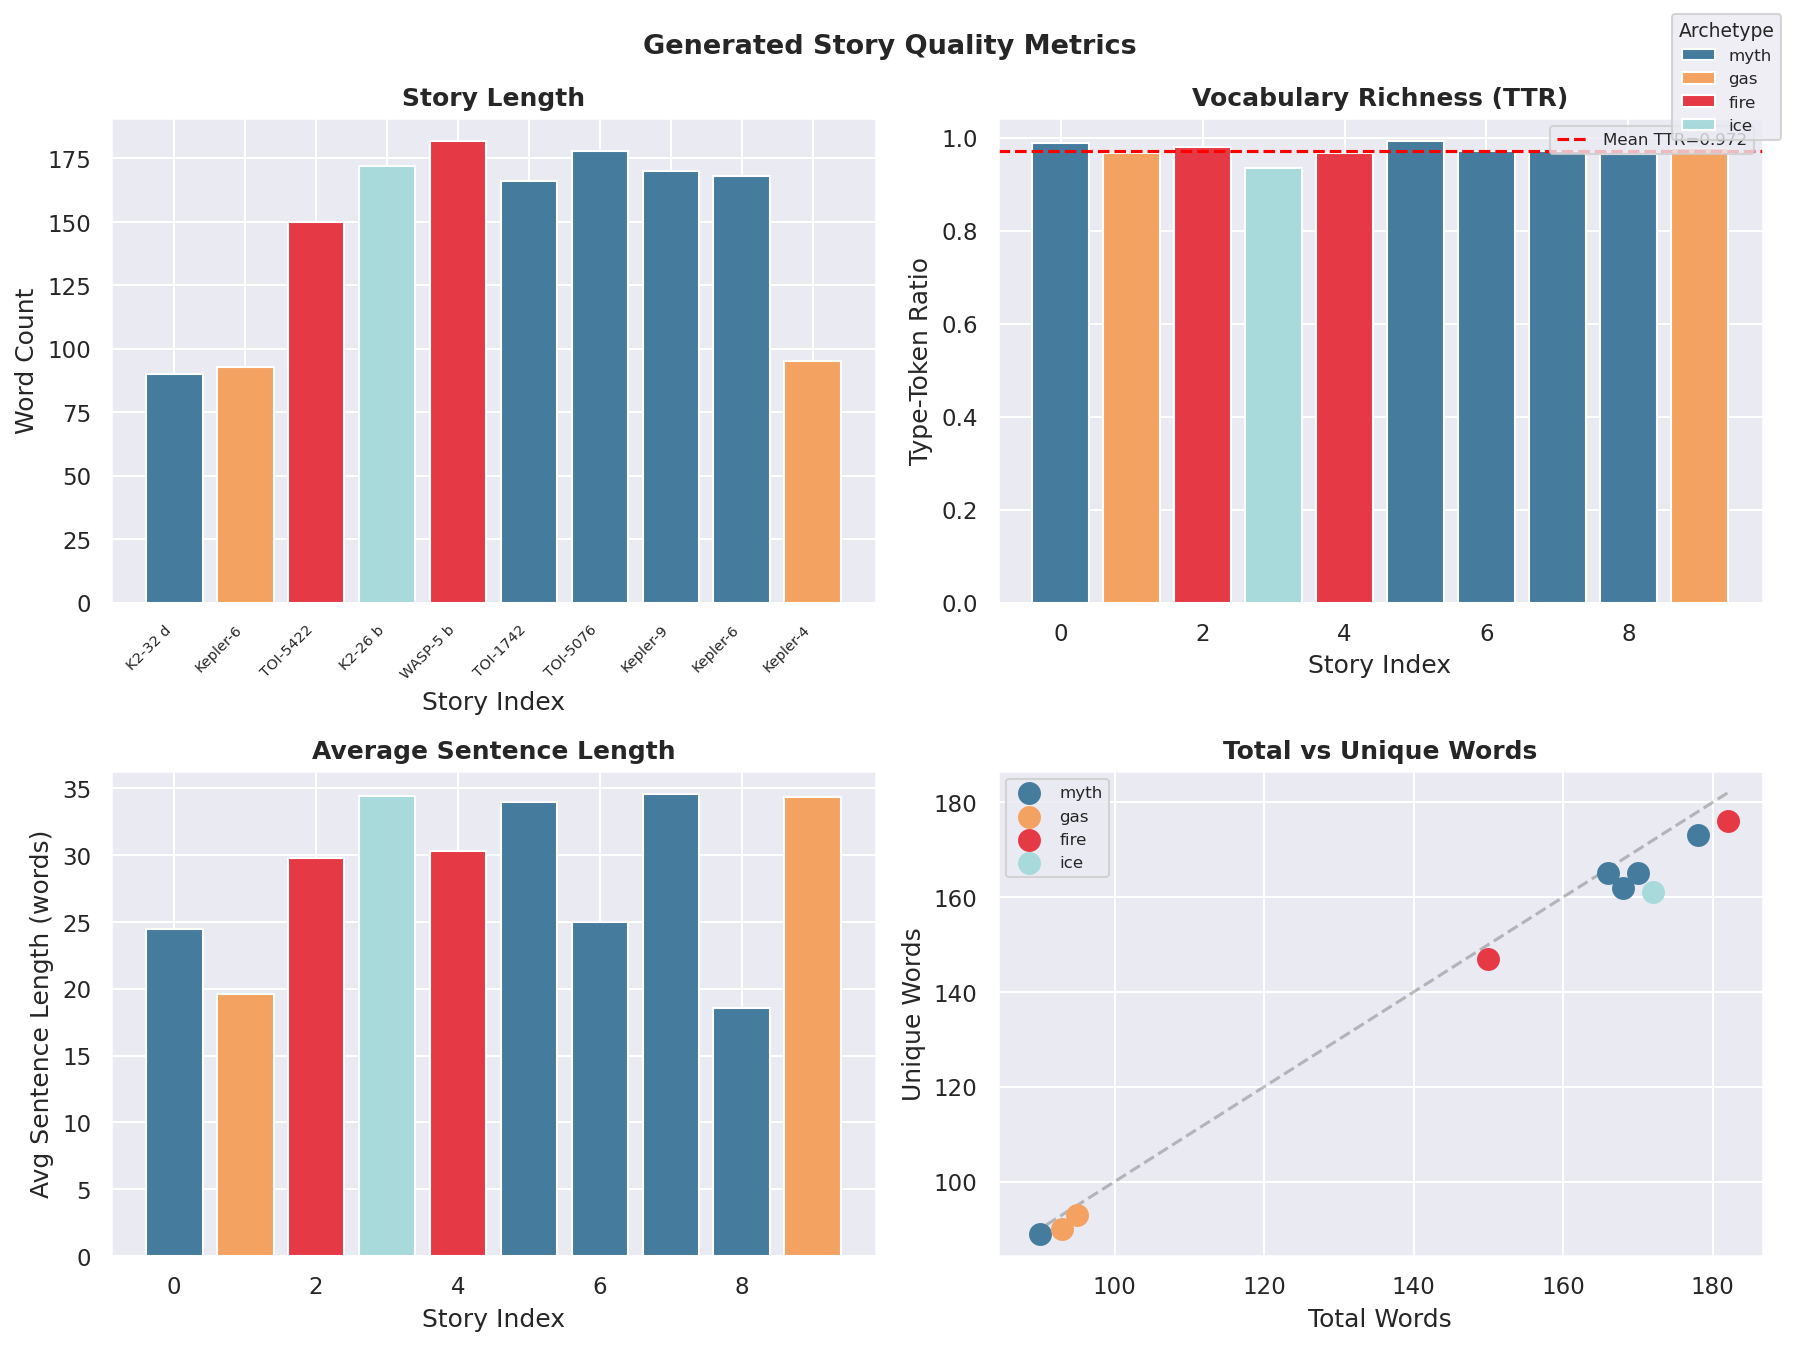
\includegraphics[width=0.8\textwidth]{images/09_story_quality.png}
    \caption{Story Quality Metrics}
\end{figure}

\section{Transformer Attention Analysis}
The attention mechanism allows GPT-2 to heavily weigh specific words in the input feature prefix when generating particular descriptions. The heatmaps below illustrate the self-attention weights.

\begin{figure}[H]
    \centering
    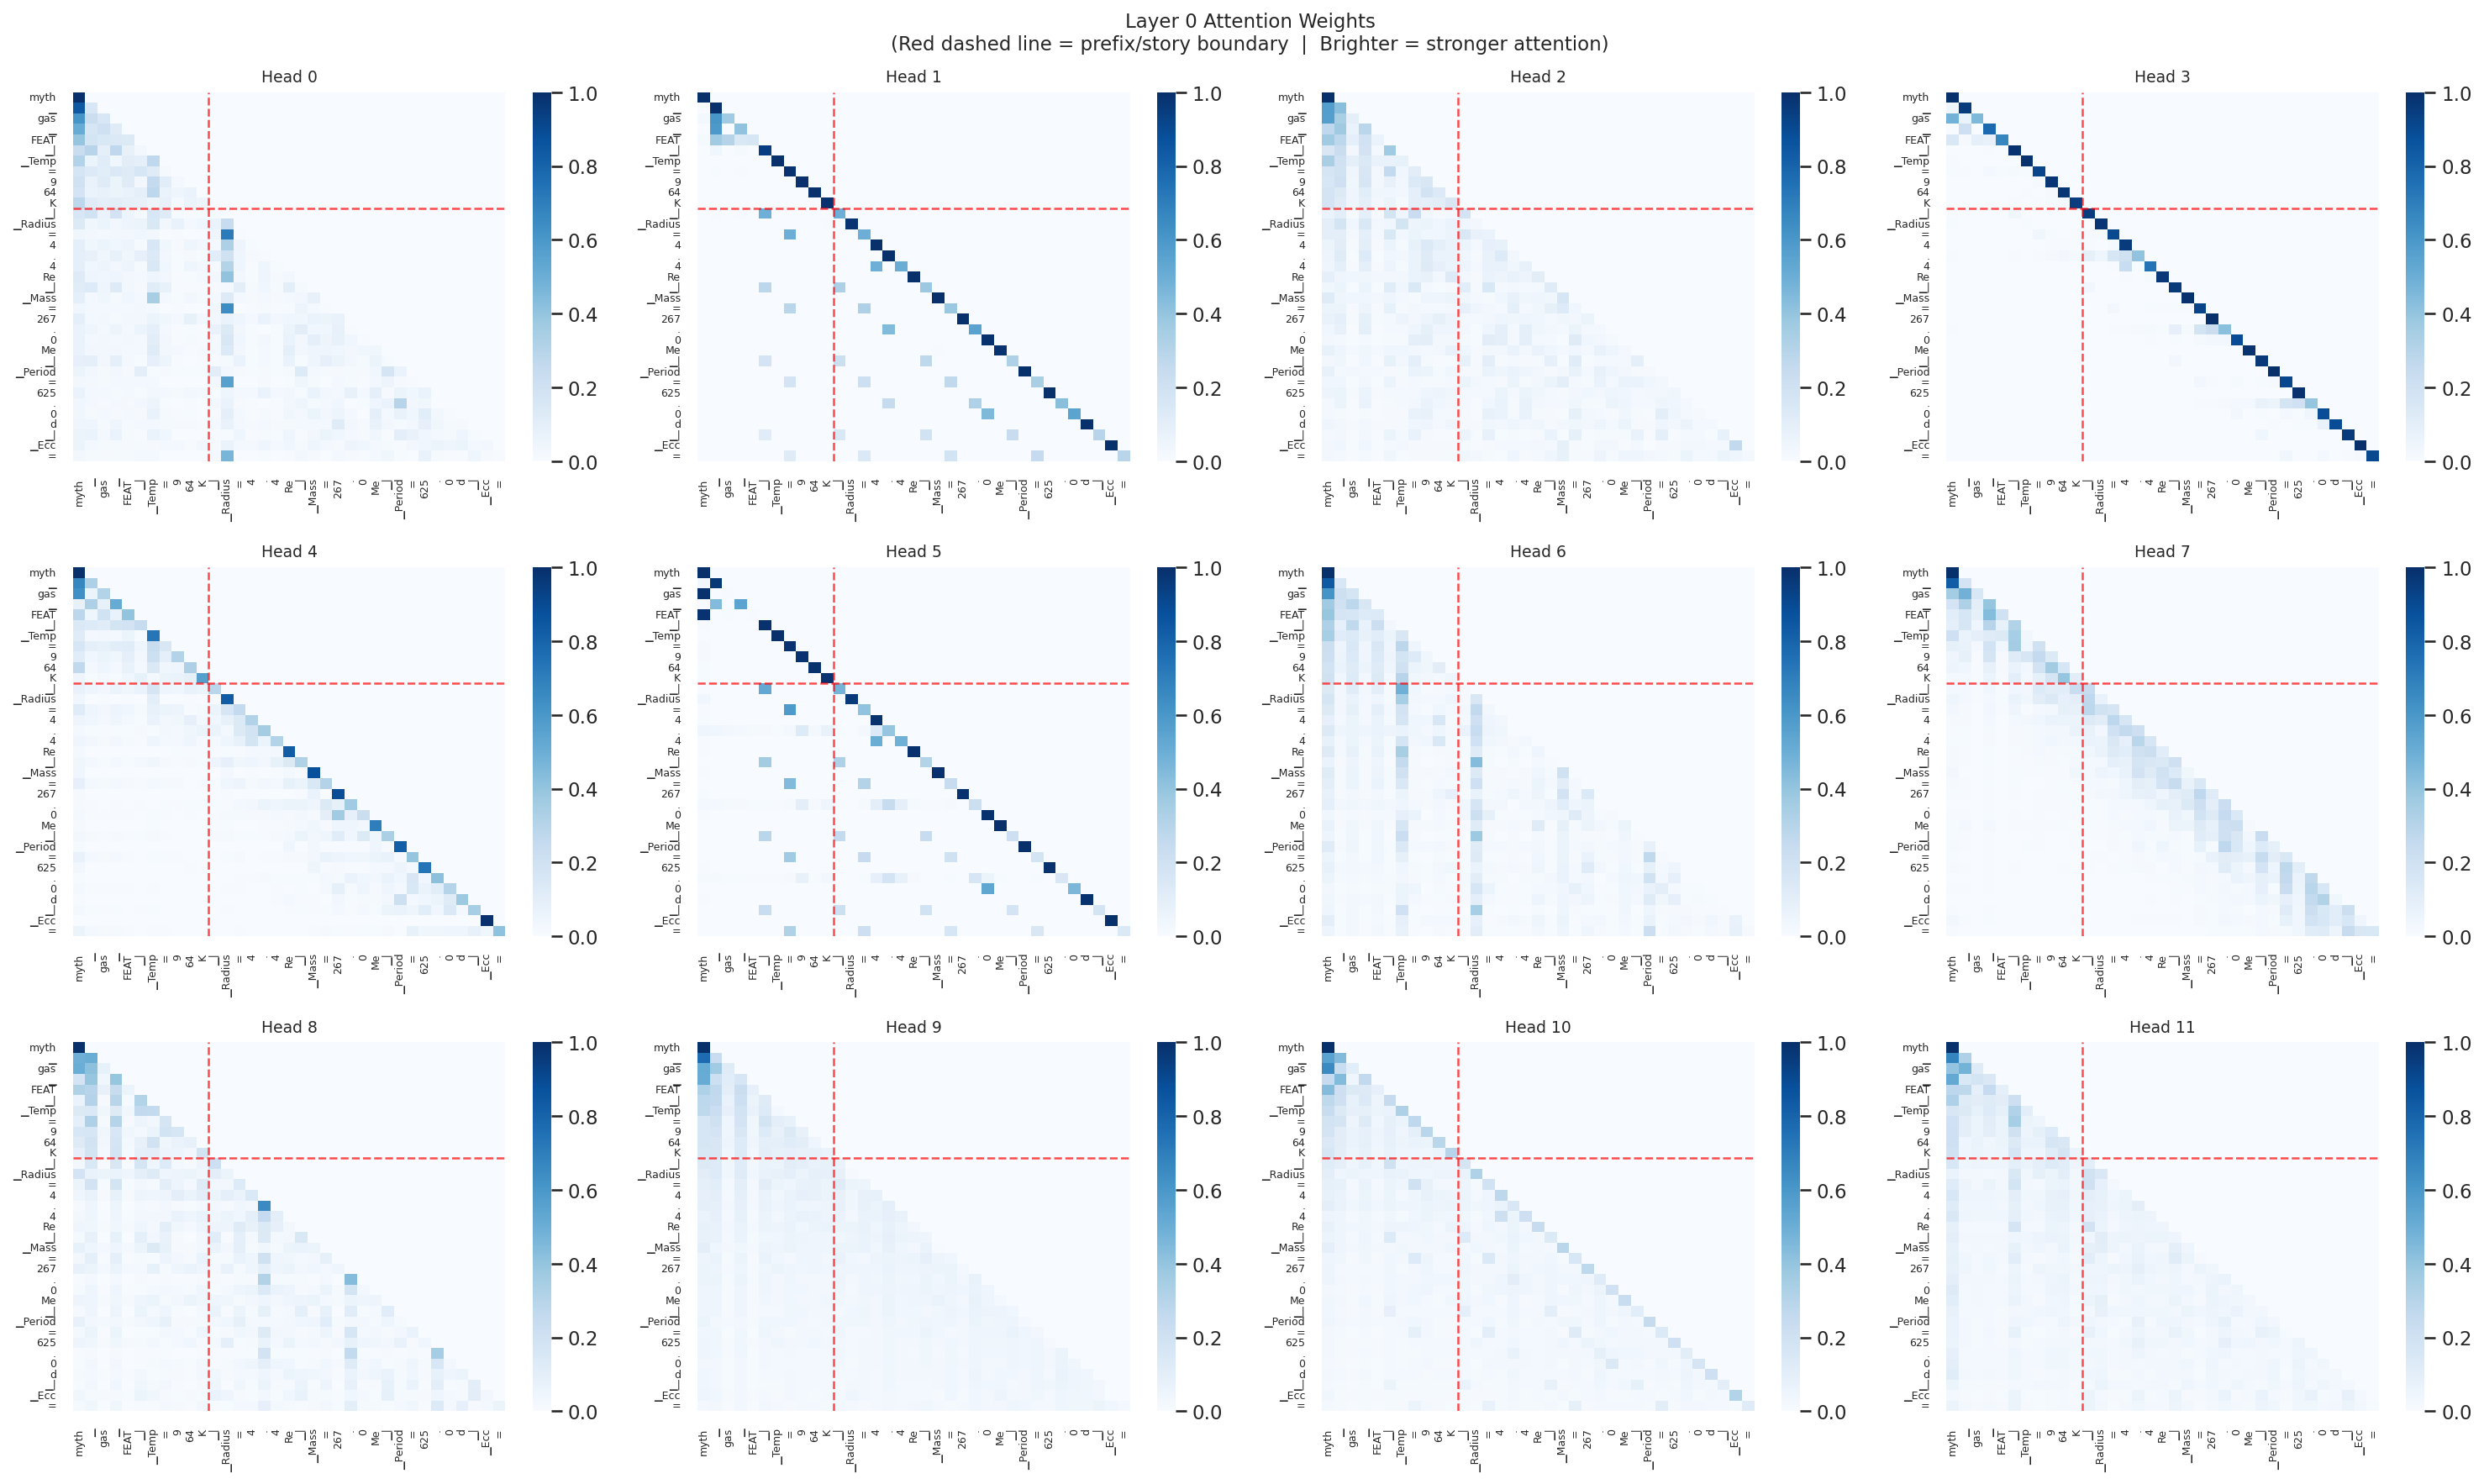
\includegraphics[width=0.48\textwidth]{images/attention_layer00.png}
    \hfill
    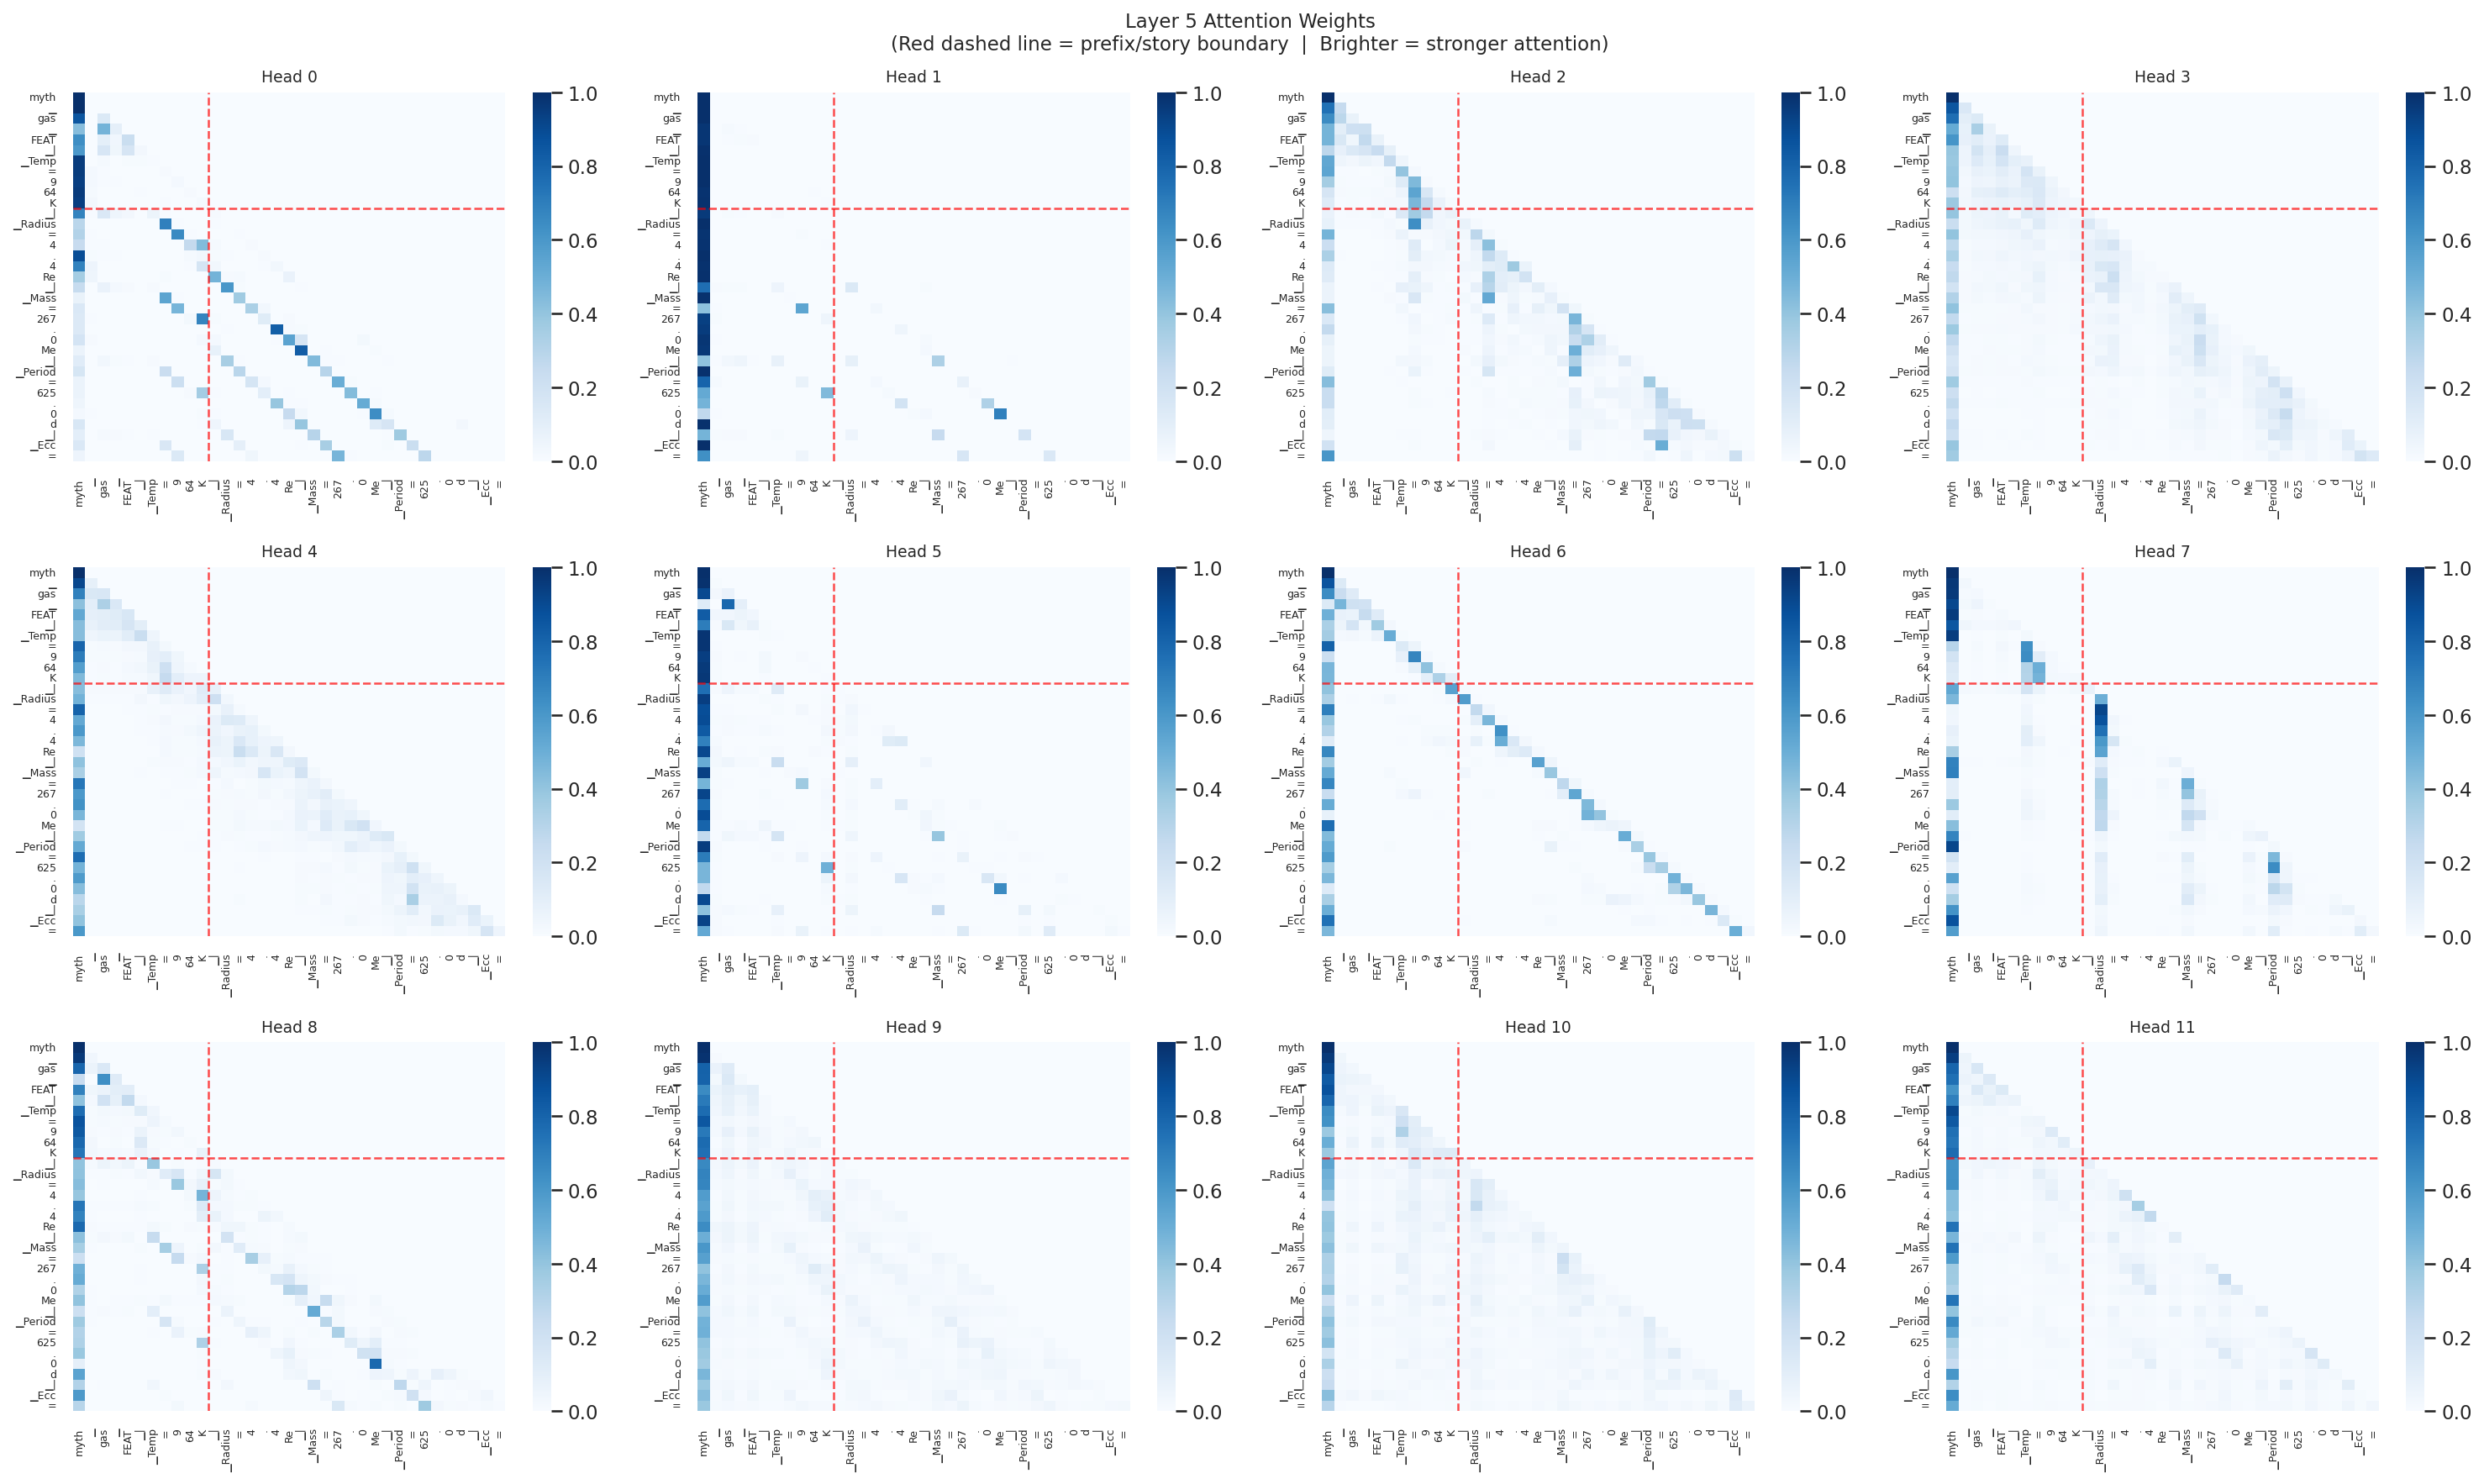
\includegraphics[width=0.48\textwidth]{images/attention_layer05.png}
    \caption{Transformer Attention Heatmaps (Layer 00 \& Layer 05)}
\end{figure}

\section{Statistical Gallery}
A broader look at the remaining statistical analyses performed on the dataset and generated outputs:

\begin{figure}[H]
    \centering
    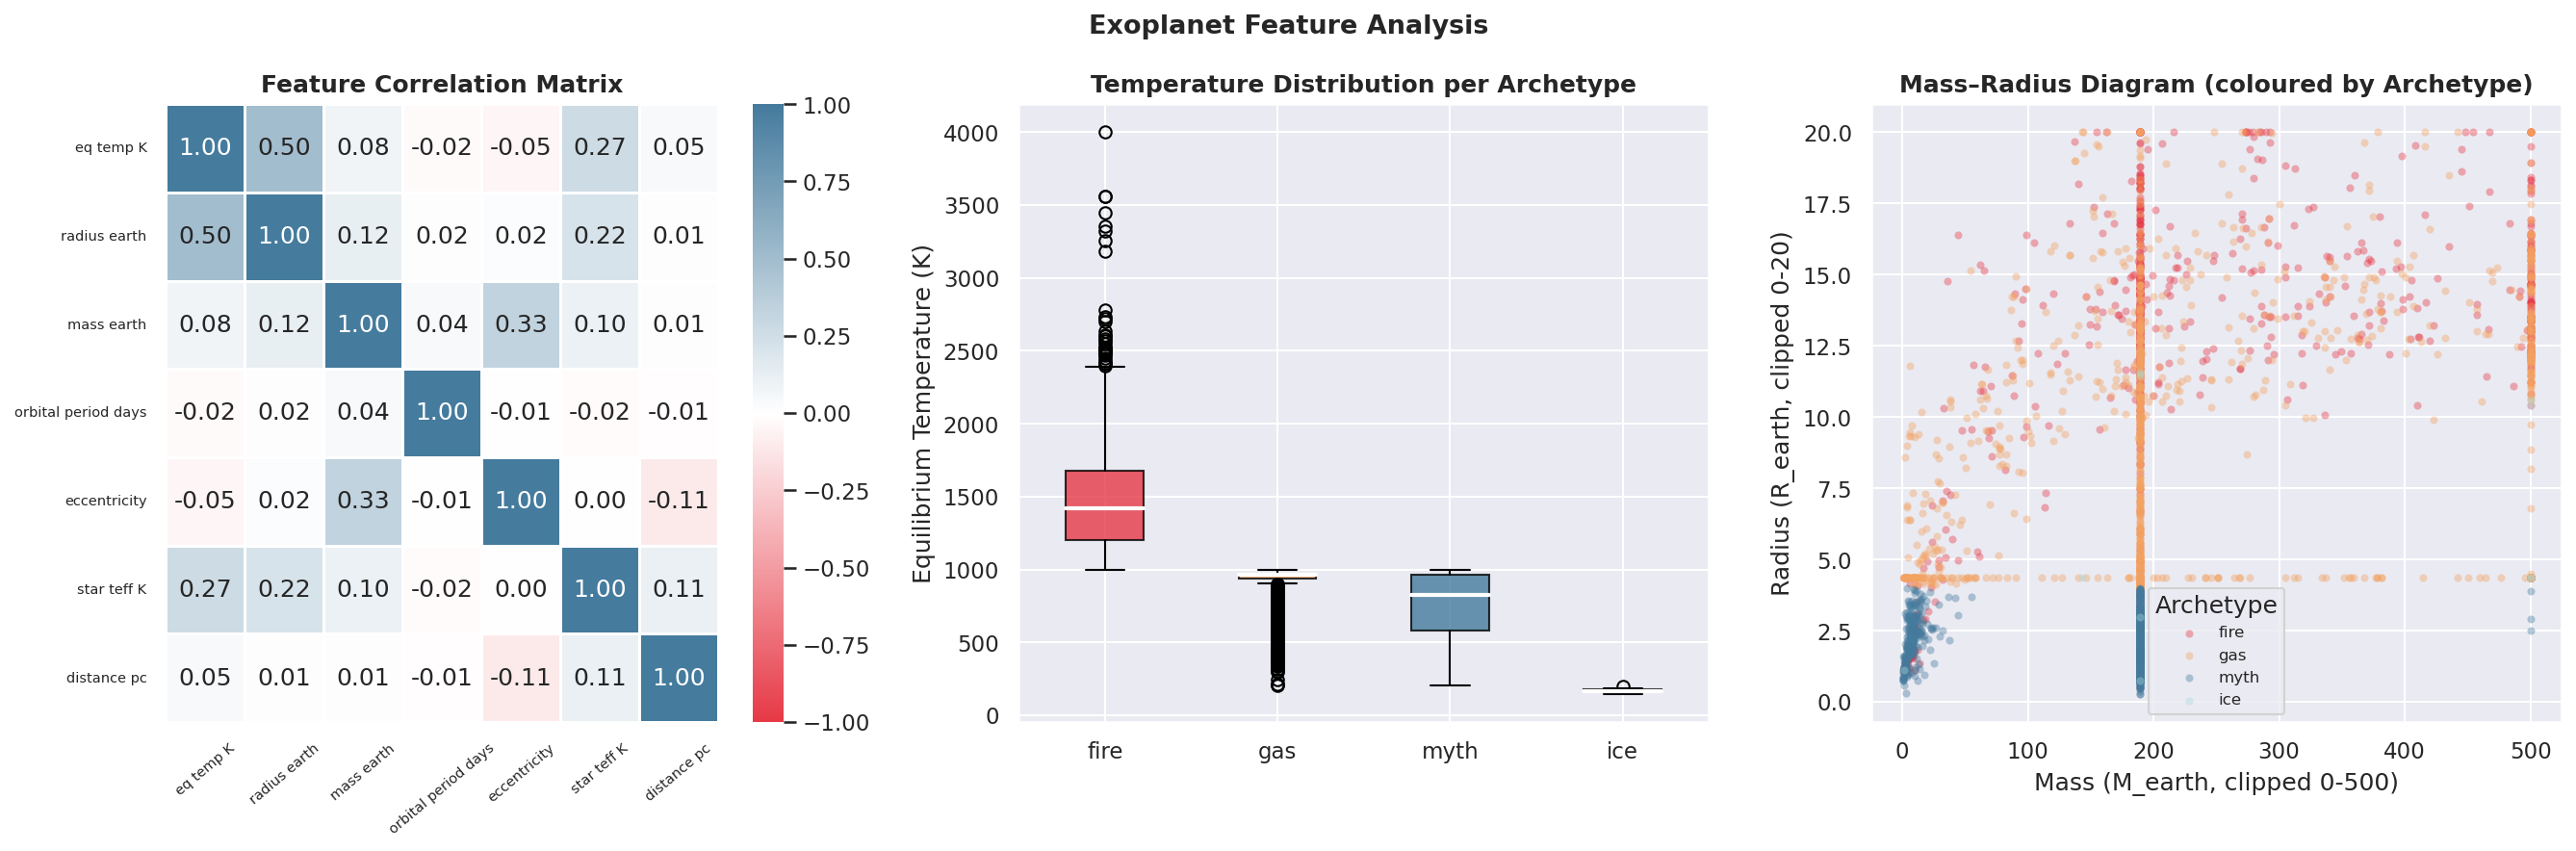
\includegraphics[width=0.48\textwidth]{images/05_feature_analysis.png}
    \hfill
    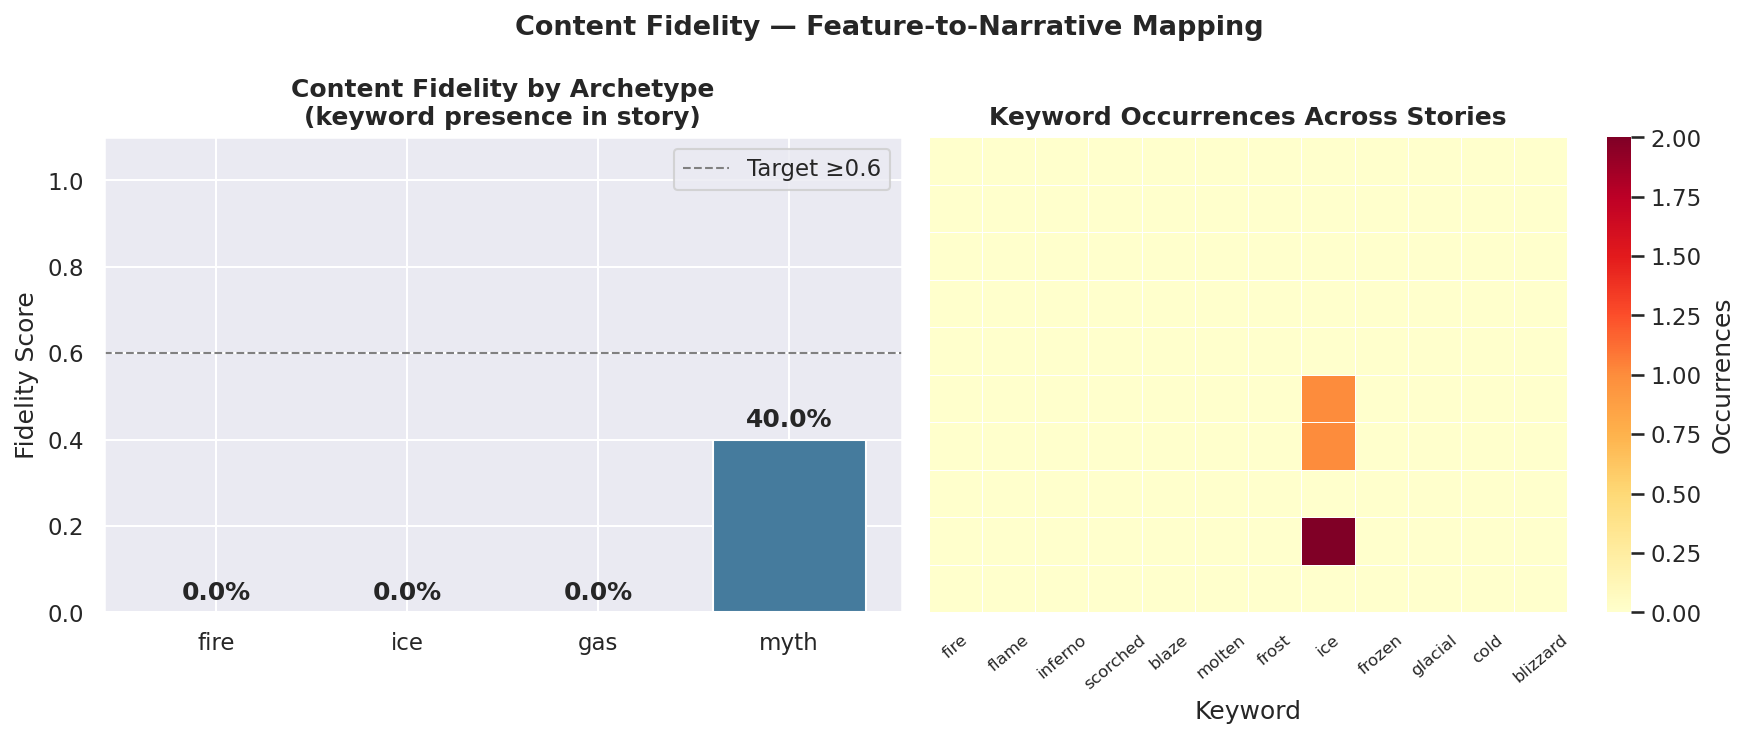
\includegraphics[width=0.48\textwidth]{images/07_content_fidelity.png}
    \caption{Feature Analysis \& Content Fidelity}
\end{figure}

\begin{figure}[H]
    \centering
    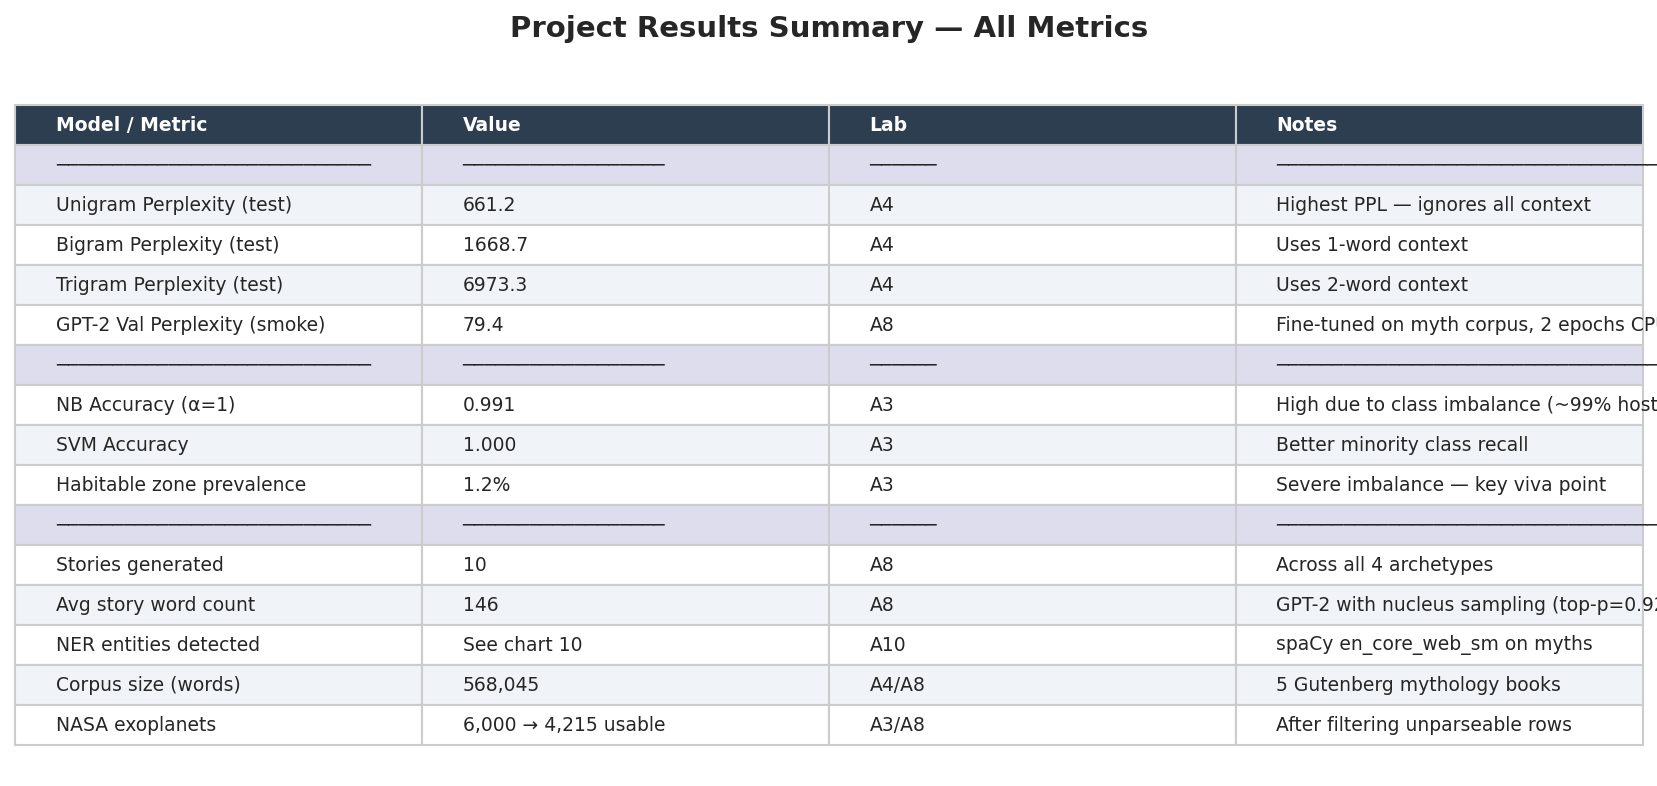
\includegraphics[width=0.48\textwidth]{images/11_summary_table.png}
    \hfill
    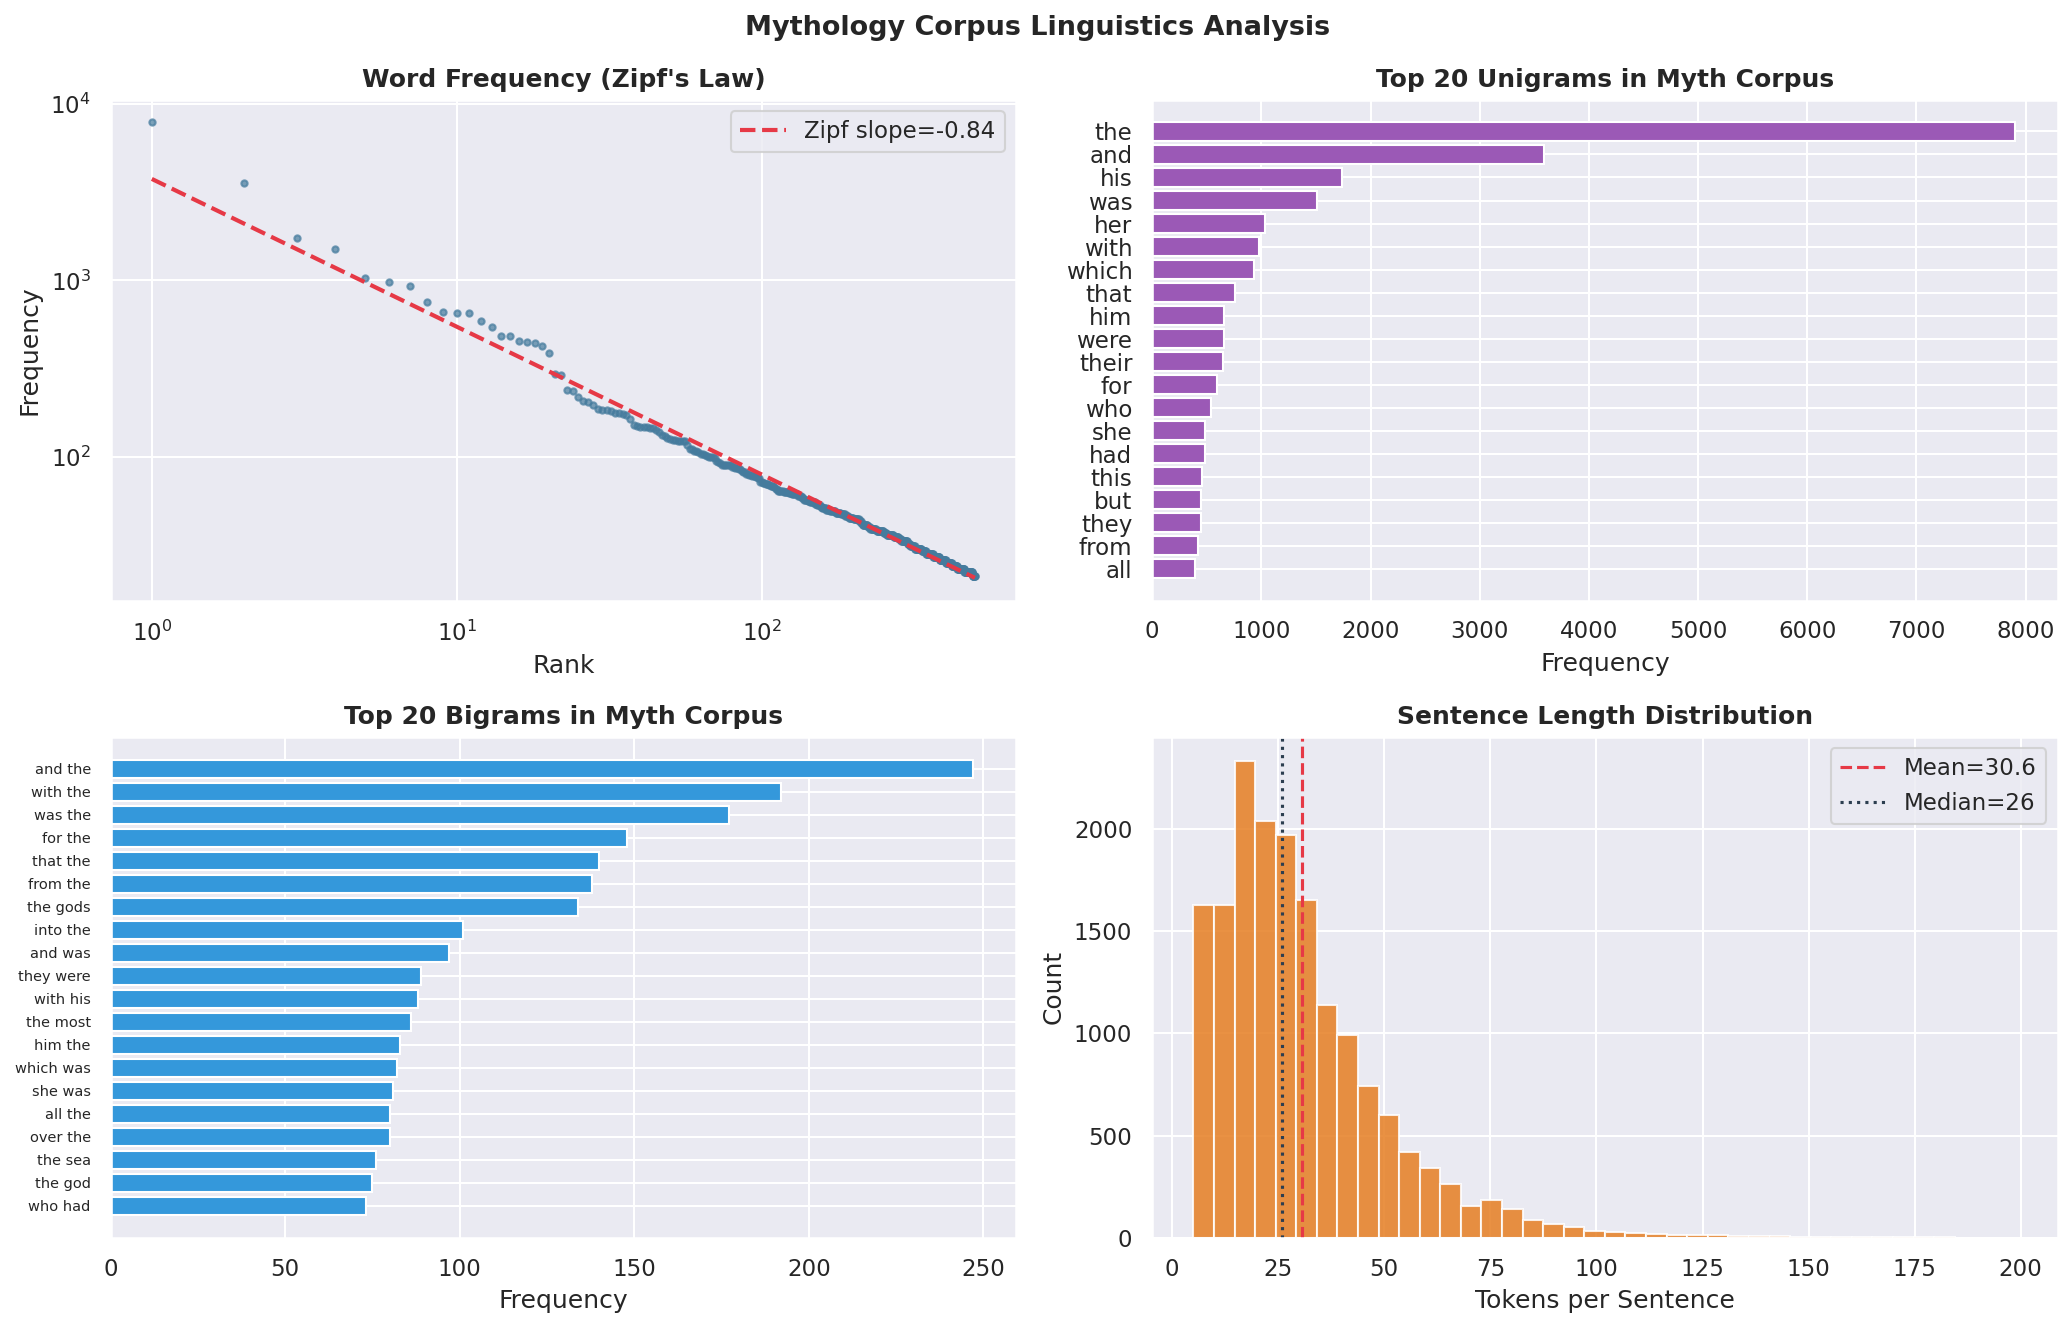
\includegraphics[width=0.48\textwidth]{images/12_corpus_linguistics.png}
    \caption{Summary Metrics \& Corpus Linguistics}
\end{figure}

% ---------------------------------------------------------
% CHAPTER 6: SUMMARY
% ---------------------------------------------------------
\chapter{Summary}
The Whispering H2 Exoplanet Mythos Generator successfully demonstrates how hard numerical data can condition continuous language models. By using a dual-conditioning architecture (text prefixes and latent variable injection) and robust sampling strategies, it bridges the domains of astrophysics and classical mythology. The classical NLP pipelines (Naïve Bayes, N-grams) serve as a critical mathematical foundation, highlighting why modern Transformer architectures with self-attention are necessary to achieve coherent, long-form narrative generation.

% ---------------------------------------------------------
% REFERENCES
% ---------------------------------------------------------
\begin{thebibliography}{9}

\bibitem{vaswani2017} 
Vaswani, Ashish, et al. 
\textit{Attention Is All You Need}. 
Advances in Neural Information Processing Systems (NeurIPS), 2017.

\bibitem{radford2019} 
Radford, Alec, et al. 
\textit{Language Models are Unsupervised Multitask Learners}. 
OpenAI, 2019.

\bibitem{holtzman2019} 
Holtzman, Ari, et al. 
\textit{The Curious Case of Neural Text Degeneration}. 
International Conference on Learning Representations (ICLR), 2020.

\bibitem{loshchilov2017} 
Loshchilov, Ilya, and Frank Hutter. 
\textit{Decoupled Weight Decay Regularization}. 
ICLR, 2019.

\bibitem{nasaexo}
NASA Exoplanet Science Institute.
\textit{NASA Exoplanet Archive}.
\url{https://exoplanetarchive.ipac.caltech.edu/}

\bibitem{gutenberg}
Project Gutenberg.
\textit{Myths and Legends Corpus}.
\url{https://www.gutenberg.org/}

\end{thebibliography}

\end{document}
